\documentclass{article}
\usepackage{amsmath, amsthm, amssymb}
\usepackage{tikz}
\usepackage{array}

\begin{document}
\section*{\huge Mathematics Homework Sheet 1}
\begin{flushright}
   \textbf{Author: Abdullah Oguz Topcuoglu}
\end{flushright}

\section*{Problem 1}
Symmetry group S will consist of rotations and reflections.
\begin{itemize}
    \item Rotations: $R_{90}$, $R_{180}$, $R_{270}$
    \item Reflections: $T_x$, $T_y$, $T_d$, $T_{d'}$
    \item Identity: $I$
\end{itemize}

% draw a square and assign numbers to the corners
\begin{center}
   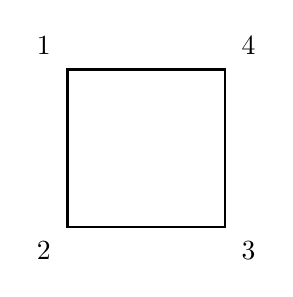
\begin{tikzpicture}
       \draw[thick] (0,0) rectangle (2,2);
       \node at (-0.3, -0.3) {2};
       \node at (2.3, -0.3) {3};
       \node at (-0.3, 2.3) {1};
       \node at (2.3, 2.3) {4};
   \end{tikzpicture}
\end{center}

$R_{i}$ rotates $i$ degrees clockwise. \\
$T_x$ reflects over the x-axis, $T_y$ reflects over the y-axis, $T_d$ reflects diagonally, and $T_{d'}$ reflects over the other diagonal.
\\
When we take a look at $S_4$, $S_4$ has 4! = 24 elements. \\
Our group S has 8 elements. \\
Lets start with identity $I$.
\begin{itemize}
   \item ()
\end{itemize}
Rotations:
\begin{itemize}
   \item $R_{90} = (1, 2, 3, 4)$
   \item $R_{180} = (1,3)(2,4)$
   \item $R_{270} = (1,4,3,2)$
\end{itemize}
Reflections:
\begin{itemize}
   \item $T_x = (1,2)(3,4)$
   \item $T_y = (1,4)(2,3)$
   \item $T_d = (1,3)$
   \item $T_{d'} = (2,4)$
\end{itemize}

So, when combined, \(S\) can be identified with this subset of \(S_4\):
\[
   \{ (), (1, 2, 3, 4), (1,3)(2,4), (1,4,3,2), (1,2)(3,4), (1,4)(2,3), (1,3), (2,4) \}
\]

\section*{Problem 2}
\section*{Problem 2(i)}
\[
   f_{a,b}(x) = ax + b
\]

\[
   (G, \diamond) = \{ f_{a,b}: a \in \mathbb{R} \setminus \{0\}, b \in \mathbb{R} \},
   f_{a,b} \diamond f_{c,d} = f_{ac, ad + b}
\]

We want to show \((G, \diamond)\) is a group. To do that, we need to show that \((G, \diamond)\) satisfies the properties of group.
\\
Associativity:
\[
   f_{a,b} \diamond (f_{c,d} \diamond f_{e,f}) = f_{a,b} \diamond f_{ce, cf + d} = f_{ace, acf + ad + b}
\]
\[
   (f_{a,b} \diamond f_{c,d}) \diamond f_{e,f} = f_{ac, ad + b} \diamond f_{e,f} = f_{ace, acf + ad + b}
\]
Thus \(f_{a,b} \diamond (f_{c,d} \diamond f_{e,f}) = (f_{a,b} \diamond f_{c,d}) \diamond f_{e,f}\).
\\
Existence of a neutral elemenet:
\[
   f_{1,0} \diamond f_{a,b} = f_{1,0} \diamond f_{a,b} = f_{a, b}
\]
\(f_{1,0}\) is the neutral element.
\\
Existence of inverses:
\[
   f_{a,b} \diamond f_{1/a, -b/a} = f_{a * (1/a), (-ab/a) + b} = f_{1, 0}
\]
Thus, \(f_{1/a, -b/a}\) is the inverse of \(f_{a,b}\).
\\
Therefore, \((G, \diamond)\) is a group.

\section*{Problem 2(ii)}
\[
   H = {f_{1,b} : b \in \mathbb{R}}
\]
We want to show \((H, \diamond)\) is a subgroup of \((G, \diamond)\) which is isomorphic to \((\mathbb{R}, +)\). \\
We need to show identity element of \((G, \diamond)\) is in \(H\):
\[
   f_{1,0} \in H
\]
We need to show \(H\) is closed under \(\diamond\) that is \(x_1,x_2 \in H \implies x_1 .x_2 \in H\):
\[
   f_{1,b_1} \diamond f_{1,b_2} = f_{1, b_1 + b_2}
\]
Thus, \(f_{1,b_1} \diamond f_{1,b_2} \in H\).
\\
We need to show \(H\) is closed under inverses that is \(x \in H \implies x^{-1} \in H\):
\[
   f_{1,b} \diamond f_{1,-b} = f_{1, 0}
\]
Thus, \(f_{1,-b} \in H\).
\\

\section*{Problem 3}
We are given \((X, .)\) is a group. We are also given that \\
(i) \(e \in X\) satisfies \(e.x = x\) for all \(x \in X\) \\
(ii) for each \(x \in X\), there exists \(x^{-1} \in X\) such that \(x^{-1}.x = e\) \\

We want to show \(x.e = x\) and \(x.x^{-1} = e\) for all \(x \in X\) \\

Proof of \(x.x^{-1} = e\):
\begin{align*}
   x^{-1}.x &= e & \text{given by (ii), multiply by e from right} \\
   (x^{-1}.x).e &= e.e & \text{associativity} \\
   x^{-1}.(x.e) &= e.e & \text{use (i)} \\
   x^{-1}.(x.e) &= e & \text{multiply by x from left} \\
   x.(x^{-1}.(x.e)) &= x.e & \text{associativity} \\
   (x.x^{-1}).(x.e) &= x.e & \text{associativity} \\
   e.(x.e) &= x.e \implies x.x^{-1} = e & \text{use (i)} \\
\end{align*}

\section*{Problem 4}
% Define the binary operations ‘subtraction’ and ‘division’ on a field (K, +, .). Let a, b, c,
% d be Elements of K with b, d 6= 0. Show that
% a
% b
% −
% c
% d
% =
% a.d − b.c
% b.d ,
% a
% b
% ,
% d
% c
% =
% a.c
% b.d,
% using only the axioms of arithmetic and your definitions

Definiton of subtraction:
\[
   a - b = a + (-b) \qquad \forall a,b \in K
\]
Thus
\[
   \frac{a}{b} - \frac{c}{d} = \frac{a}{b} + \left(-\frac{c}{d}\right)
\]

Definition of division:
\[
   \frac{a}{b} = a \cdot b^{-1} \qquad \forall a,b \in K
\]

\[
   \frac{a}{b} = \frac{a \cdot d}{b \cdot d}, \quad \frac{c}{d} = \frac{c \cdot b}{d \cdot b}
\]
Multiplying by a value and its inverse does not change the value of the fraction.
\[
   \frac{a}{b} - \frac{c}{d} = \frac{a \cdot d}{b \cdot d} + \left(-\frac{c \cdot b}{d \cdot b}\right) \qquad \text{(defition of subtraction)}
\]
\[
   = \frac{a \cdot d - c \cdot b}{b \cdot d}
\]
\\
\\
\\
We want to show that
\[
   \frac{\frac{a}{b}}{\frac{d}{c}} = \frac{a.c}{b.d}
\]

\begin{align*}
   \frac{\frac{a}{b}}{\frac{d}{c}} &= \frac{a}{b} \cdot \left(\frac{d}{c}\right)^{-1} & \text{(definition of division)} \\
                                   &= a.b^{-1}.(d.c^{-1})^{-1} & \text{(defitiniton of division)} \\
                                   &= a.b^{-1}.c.d^{-1} & \text{(inverse of . operation from field axioms)} \\
                                   &= a.c.b^{-1}.d^{-1} & \text{(commutativity)} \\
                                   &= (a.c).(b^{-1}.d^{-1}) & \text{(associativity)} \\
                                   &= \frac{ac}{b.d} & \text{(definition of division)} \\
\end{align*}

Thus, we have shown that
\[
   \frac{a}{b} - \frac{c}{d} = \frac{a.d - b.c}{b.d}
\]
\[
   \frac{\frac{a}{b}}{\frac{d}{c}} = \frac{a.c}{b.d}
\]

\section*{Problem 5}
% Show that {a + b
% √
% 2 : a, b ∈ Q} is a subfield of (R, +, .).

We want to show that
\[
   S := \{a + b\sqrt{2} : a, b \in \mathbb{Q}\}
\]
is a subfield of \((\mathbb{R}, +, \cdot)\). \\
\\
S is closed with respect to + and .:
\begin{align*}
   (a + b\sqrt{2}) + (c + d\sqrt{2}) &= (a + c) + (b + d)\sqrt{2} \\
   (a + b\sqrt{2})(c + d\sqrt{2}) &= ac + ad\sqrt{2} + bc\sqrt{2} + bd(2) \\
                                   &= (ac + 2bd) + (ad + bc)\sqrt{2}
\end{align*}
\\
\\
S contains the identity elements of + and .:
\begin{align*}
   0 &= 0 + 0\sqrt{2} \\
   1 &= 1 + 0\sqrt{2}
\end{align*}
\\
\\
S contains the inverses of + and .:
\begin{align*}
   -(a + b\sqrt{2}) &= -a - b\sqrt{2} \\
   (a + b\sqrt{2})^{-1} &= \frac{1}{a + b\sqrt{2}} \cdot \frac{a - b\sqrt{2}}{a - b\sqrt{2}} \\
                        &= \frac{a - b\sqrt{2}}{a^2 - 2b^2} \\
                        &= \frac{a}{a^2 - 2b^2} - \frac{b}{a^2 - 2b^2}\sqrt{2}
\end{align*}

We have shown that \(S\) is closed with respect to + and ., contains the identity elements of + and ., and contains the inverses of + and .. \\
Therefore, \((S, +, .)\) is a subfield of \((\mathbb{R}, +, \cdot)\).


\end{document}